This section is divided into two subsections. First we present the results of manual experiments that we obtained by hand via the UI that we implemented in section \ref{sec:manualver}.
The second section \ref{sec:autover} contains results we obtained and evaluated automatically by running the simulations headlessly.

\subsection{Manual Verifications}
\label{sec:manualver}
This experiment was used to prove that the setup we built could find the shortest path in the three mentioned maps. For each map we tested how much time or steps it took to find an optimized path, How much creeps were created to find the path and how much of them arrived at the end point before the shortest path was found. We did not only test this with the basic ACO algorithm but also with the weighted shortest path algorithm to see if the results would be different. For every map we ran the experiment five times to see what the average result would be so that one irregular result would not influence our end result. Every time we ran the experiment until a pheromone level of 0.8 was reached in a path.
The results of the experiment can be found in figure \ref{fig:manres}. The following text contains the conclusion we have drawn from that table.

Overall we found out that it was possible for any of our creep behaviors  to find a path and sometimes even the shortest. In the first map with an obviously shorter path it took about 30 iterations for the shortest path only to fully reinforce the optimized path. In this map the weighted shortest path algorithm had about the same results. In the second map where no obvious shortest path was present because there were two shortest paths it took the shortest path only an average of 43 ticks to the point that one path was fully optimized. Here the weighted shortest path took much longer because the pheromones on both paths would keep getting increased by a little.  

In the third, more complicated maze map there started to be instances where the optimal route would not be found or would be longer than the real shortest path when. This had several reasons. The first reason we found is that the decay of pheromones would already take too much of the pheromones away before the next wave would reach the path. When we took this decay away waves started going in loops because they would start reinforcing themselves. This problem was the biggest while using the weighted ACO algorithm. Because of the bigger complexity of the map there would also be a chance that a wrong path would already get reinforced before all routes were tried. The time also took longer with an average of 79 ticks before an optimum was found. With the weighted algorithm sometimes the found path was not necessarily the shortest path.

After we added towers to the maps we noticed that the results were very similar with amounts of time it took to reach an optimum, depending on how the towers were placed. As expected it did take more creeps because many of them died. In the basic algorithm no pheromones were added when creeps did not reach the end of the path. This meant that creeps would find routes around the towers when the creeps would not be able to get through and even when they did there would be way more using the longer routes. When it was less obvious which path was the best because we placed multiple towers it would take longer to create an optimum.

\begin{figure}[H]
	\begin{tabular}{|l|l|l|l|l|l|}
	\hline
		Simple 2 way path ACO    & test 1 & test 2 & test 3 & test 4 & test 5 \\\hline
		Time until optimized     & 30     & 25     & 33     & 29     & 30     \\
		Amount of creeps spawned & 199    & 206    & 184    & 211    & 197    \\
		Amount of creeps arrived & 111    & 111    & 106    & 107    & 112    \\
	\hline
		Simple 2 way path ACO weighted & test 1 & test 2 & test 3 & test 4 & test 5 \\ \hline
		Time until optimized           & 27     & 30     & 30     & 31     & 33     \\
		Amount of creeps spawned       & 220    & 211    & 206    & 221    & 197    \\
		Amount of creeps arrived       & 105    & 106    & 116    & 113    & 105    \\\hline
		Intermediate 4 way path ACO & test 1 & test 2 & test 3 & test 4 & test 5 \\\hline
		Time until optimized        & 39     & 50     & 37     & 36     & 53     \\
		Amount of creeps spawned    & 251    & 345    & 237    & 288    & 325    \\
		Amount of creeps arrived    & 117    & 157    & 110    & 135    & 149    \\\hline
		
		Intermediate 4 way path ACO weighted & test 1 & test 2 & test 3 & test 4 & test 5 \\\hline
		Time until optimized                 & 46     & 95     & 47     & 51     & 55     \\
		Amount of creeps spawned             & 335    & 717    & 318    & 325    & 379    \\
		Amount of creeps arrived             & 135    & 290    & 133    & 142    & 157    \\\hline
		
		Maze path ACO & test 1 & test 2 & test 3 & test 4 & test 5 \\\hline
		Time until optimized      & 78     & 76     & 104    & 75     & 62     \\
		Amount of creeps spawned  & 451    & 546    & 727    & 559    & 467    \\
		Amount of creeps arrived  & 170    & 236    & 327    & 243    & 148    \\\hline
		
		Maze path ACO weights & test 1 & test 2 & test 3 & test 4 & test 5 \\\hline
		Time until optimized              & 78     & 76     & 57     & 52     & 48     \\
		Amount of creeps spawned          & 397    & 440    & 369    & 372    & 368    \\
		Amount of creeps arrived          & 98     & 102    & 100    & 96     & 96     \\\hline
	\end{tabular}
	\label{fig:manres}
	\caption{Results of our manual verification organized in a table}
\end{figure}


\subsection{Automatic Evaluation Results}
\label{sec:autover}
For the automatic evaluation we tried varying settings and ran them across all maps. Because the amount of different parameters and the hence large amount of graphs to interpret we will here only mention and display the settings that we deemed relevant information. To be statistically relevant every experiment setting is run 50 times and we then take the mean value of that for the graph. We also always include Towers in the maps.

Regarding the settings when we talk about normal settings, then these are the settings we found to work best using the manual mode. This consist of a spawn-amount of 14, a decay-threshold of -0.007 and a pheromone-increase threshold of 0.01.

First of we will start out by excluding the continuous vapor in the future Figures because as Figure \ref{fig:mirrorvaptick} clearly shows, the runtime is much larger than for all other three behaviors for the mirrored map. This behavior was visible across all maps and settings, another example that stresses the uselessness of the continuous vapor is the runtime graph portrayed in Figure \ref{fig:shortlongvaptick} for the short and long map, the very basic map that all of them should be able to easily master.

\begin{figure}[H]
  \centering
  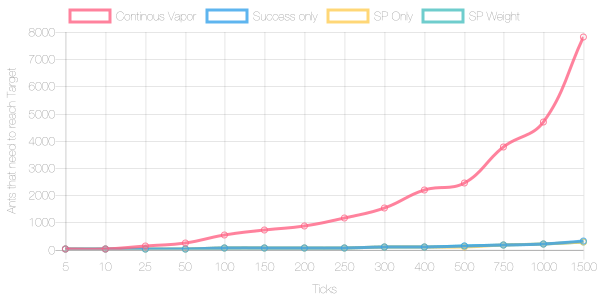
\includegraphics[width=1\linewidth]{images/normalmirroredwithtower-ticks-line}
  \caption{Comparing required Tick-Amount on the y-Axis to the target amount of creeps to reach the target on the x-Axis for the mirrored map with normal settings.}
  \label{fig:mirrorvaptick}
\end{figure}

\begin{figure}[H]
  \centering
  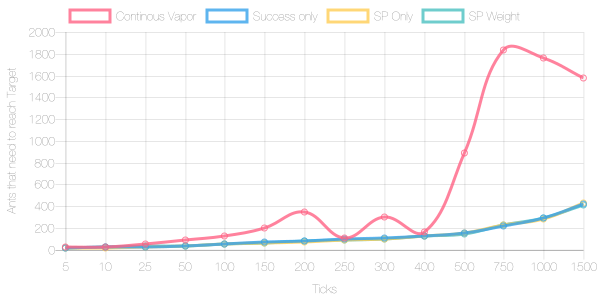
\includegraphics[width=1\linewidth]{images/normalshortandlongwithtowers-ticks-line}
  \caption{Comparing required Tick-Amount on the y-Axis to the target amount of creeps to reach the target on the x-Axis for the short and long map with normal settings}
  \label{fig:shortlongvaptick}
\end{figure}

With the automatic evaluation we also further prove, that deducing pheromones upon death is rather counter-productive than helpful as visible in Figure \ref{fig:deathsubshitty}. But it does make sense given that any street-part a creep crossed on it's way to death will be deduced in pheromone. That means even a correct path like in the short and long map the longer one can lead to pheromone deduction and hence make the path unattractive again and future creeps more likely to walk the even more dangerous path with more deaths.
Also for the weighted shortest path leaving death-substraction out even slightly improves the result. As for the non continuous vapor behavior, not only does substraction not matter as much, but also all three perform quite similar.


\begin{figure}[H]
  \centering
  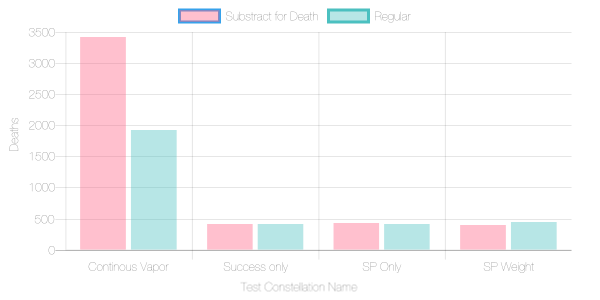
\includegraphics[width=1\linewidth]{images/normalshortandlongwithtowers-deaths}
  \caption{Comparing deaths for the different creep behaviors with and without substracting pheromones upon death on the short and long map with normal settings}
  \label{fig:deathsubshitty}
\end{figure}

The following graph, depicted in Figure \ref{fig:threesame} which doesn't include the continuous vapor any more shows, shows that the remaining three behaviors perform similar not only regarding death amount but also regarding their runtime.

\begin{figure}[H]
  \centering
  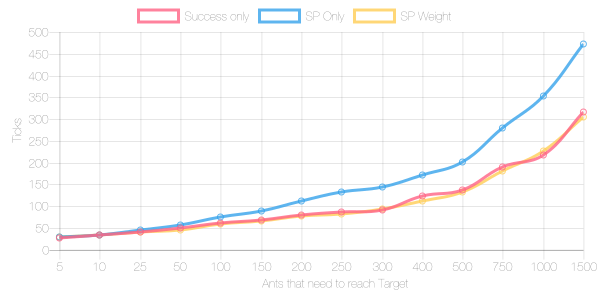
\includegraphics[width=1\linewidth]{images/normalsquaremaze-ticks-line}
  \caption{Comparing required Tick-Amount on the y-Axis to the target amount of creeps to reach the target on the x-Axis for the maze map with normal settings}
  \label{fig:threesame}
\end{figure}

Because of that similarity we ran another experiment only using the shortest weighted path algorithm, but with a few differing settings. The result of that is accessible through Figure \ref{fig:diffsettings} which portrays the amount of Ticks and Figure \ref{fig:diffsettingsdeath} which displays the amount of deaths.

As we can see using a high spawn rate with no or low decay will result in much more deaths than usual. Manually reconstructing this scenario with the UI explains why that is: With a high spawn rate many creeps come through every way regardless of the tower strength. Hence bad ways can be reinforced and made attractive even though they are not.
Another possible conclusion is that using a low spawn rate in combination with no or low decay will increase runtime, which is logical given that the target is the amount of creeps that need to reach the target and less spawned creeps mean less creeps per tick are able to arrive at the target. 

\begin{figure}[H]
  \centering
  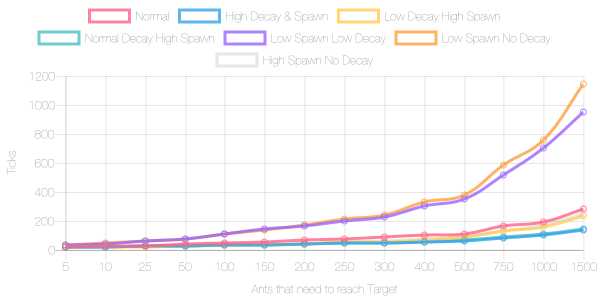
\includegraphics[width=1\linewidth]{images/mirroredwithtower-ticks-line}
  \caption{Comparing required Tick-Amount on the y-Axis to the target amount of creeps to reach the target on the x-Axis for the mirrored map with normal settings}
  \label{fig:diffsettings}
\end{figure}

\begin{figure}[H]
  \centering
  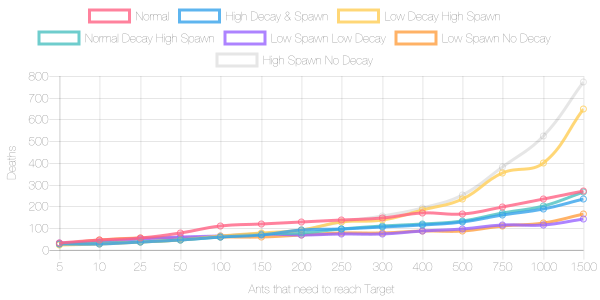
\includegraphics[width=1\linewidth]{images/mirroredwithtower-deaths-line}
  \caption{Comparing amount of deaths on the y-Axis to the target amount of creeps to reach the target on the x-Axis for the mirrored map with normal settings}
  \label{fig:diffsettingsdeath}
\end{figure}

We have also already shown that the spawn-amount only has a logical impact on the tick amount and 14 is a good number given the damage of the towers. Now we also want to prove that the pheromone increase and decrease-level we declared as \textit{normal} are optimal
For that Figure \ref{fig:diffsettings2} compares the amount of ticks and Figure \ref{fig:diffsetting2sdeath} the amount of deaths for different pheromone-settings with the spawn amount 14 on the mirrored map.

As we can see the best value is in both instances achieved by the completely normal settings. It also shows that a low increase or also decay can negatively influence runtime. Also using a low pheromone increase can cause more deaths.

\begin{figure}[H]
  \centering
  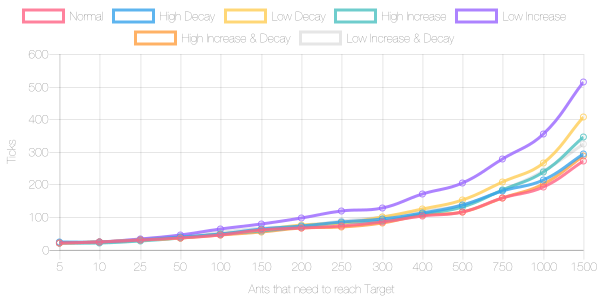
\includegraphics[width=1\linewidth]{images/mirrorednormalpheromticks}
  \caption{Comparing required Tick-Amount o n the y-Axis to the target amount of creeps to reach the target on the x-Axis for the mirrored map with varying settings}
  \label{fig:diffsettings2}
\end{figure}

\begin{figure}[H]
  \centering
  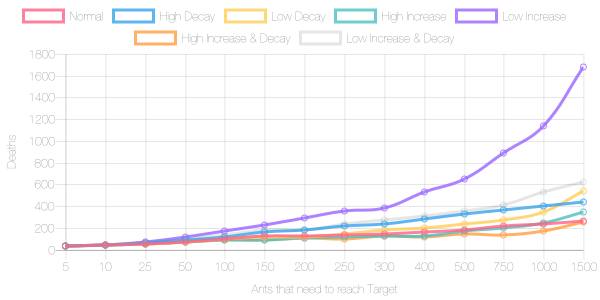
\includegraphics[width=1\linewidth]{images/mirroredwittowerdeaths}
  \caption{Comparing amount of deaths on the y-Axis to the target amount of creeps to reach the target on the x-Axis for the mirrored map with normal settings}
  \label{fig:diffsetting2sdeath}
\end{figure}